%%
%% This is file `sample-sigconf.tex',
%% generated with the docstrip utility.
%%
%% The original source files were:
%%
%% samples.dtx  (with options: `sigconf')
%% 
%% IMPORTANT NOTICE:
%% 
%% For the copyright see the source file.
%% 
%% Any modified versions of this file must be renamed
%% with new filenames distinct from sample-sigconf.tex.
%% 
%% For distribution of the original source see the terms
%% for copying and modification in the file samples.dtx.
%% 
%% This generated file may be distributed as long as the
%% original source files, as listed above, are part of the
%% same distribution. (The sources need not necessarily be
%% in the same archive or directory.)
%%
%% The first command in your LaTeX source must be the \documentclass command.
\documentclass[sigconf]{acmart}

\settopmatter{printacmref=false} % Removes citation information below abstract
\renewcommand\footnotetextcopyrightpermission[1]{} % removes footnote with conference information in first column
\pagestyle{plain} % removes running headers
\usepackage{listings}
\usepackage{color}

\definecolor{dkgreen}{rgb}{0,0.6,0}
\definecolor{gray}{rgb}{0.5,0.5,0.5}
\definecolor{mauve}{rgb}{0.58,0,0.82}

\lstset{frame=tb,
  language=Python,
  aboveskip=3mm,
  belowskip=3mm,
  showstringspaces=false,
  columns=flexible,
  basicstyle={\small\ttfamily},
  numbers=none,
  numberstyle=\tiny\color{gray},
  keywordstyle=\color{blue},
  commentstyle=\color{dkgreen},
  stringstyle=\color{mauve},
  breaklines=true,
  breakatwhitespace=true,
  tabsize=3
}

%%
%% \BibTeX command to typeset BibTeX logo in the docs
\AtBeginDocument{%
  \providecommand\BibTeX{{%
    \normalfont B\kern-0.5em{\scshape i\kern-0.25em b}\kern-0.8em\TeX}}}

%% Rights management information.  This information is sent to you
%% when you complete the rights form.  These commands have SAMPLE
%% values in them; it is your responsibility as an author to replace
%% the commands and values with those provided to you when you
%% complete the rights form.

%%
%% Submission ID.
%% Use this when submitting an article to a sponsored event. You'll
%% receive a unique submission ID from the organizers
%% of the event, and this ID should be used as the parameter to this command.
%%\acmSubmissionID{123-A56-BU3}

%%
%% The majority of ACM publications use numbered citations and
%% references.  The command \citestyle{authoryear} switches to the
%% "author year" style.
%%
%% If you are preparing content for an event
%% sponsored by ACM SIGGRAPH, you must use the "author year" style of
%% citations and references.
%% Uncommenting
%% the next command will enable that style.
%%\citestyle{acmauthoryear}

%%
%% end of the preamble, start of the body of the document source.
\begin{document}

%%
%% The "title" command has an optional parameter,
%% allowing the author to define a "short title" to be used in page headers.
\title{Final Report of BAAI-ZHIHU Expert Finding Competition}

%%
%% The "author" command and its associated commands are used to define
%% the authors and their affiliations.
%% Of note is the shared affiliation of the first two authors, and the
%% "authornote" and "authornotemark" commands
%% used to denote shared contribution to the research.
\author{Baodi Shan}

\email{lwshanbd@gmail.com}
\orcid{1234-5678-9012}

\affiliation{%
  \institution{Shandong University}
  \streetaddress{JimoDistrict BinhaiRoad 72}
  \city{Qingdao}
  \country{China}
  \postcode{266237}
}









%%
%% By default, the full list of authors will be used in the page
%% headers. Often, this list is too long, and will overlap
%% other information printed in the page headers. This command allows
%% the author to define a more concise list
%% of authors' names for this purpose.
\renewcommand{\shortauthors}{Trovato and Tobin, et al.}

%%
%% The abstract is a short summary of the work to be presented in the
%% article.
\begin{abstract}
   Knowledge sharing services have become one of the most important and popular applications on the global Internet. Therefore, how to connect knowledge, experts and users, and increase the willingness of experts to respond has become the central topic of knowledge sharing services. In this competition we will do something to solve this problem. In this process, I used assemble learning, XGboost and LGBM. At the same time, feature extraction is also a 	brightened dot of my work.
\end{abstract}

%%
%% The code below is generated by the tool at http://dl.acm.org/ccs.cfm.
%% Please copy and paste the code instead of the example below.
%%


%%
%% Keywords. The author(s) should pick words that accurately describe
%% the work being presented. Separate the keywords with commas.
\keywords{Knowledge Sharing, Datamining, XGboost, LGBM}

%% A "teaser" image appears between the author and affiliation
%% information and the body of the document, and typically spans the
%% page.


%%
%% This command processes the author and affiliation and title
%% information and builds the first part of the formatted document.
\maketitle

\section{Introduction AND Background}
This competition is one of in the Beijing Academy of Artificial Intelligence’s 10 AI competitions in 2019.

 
Knowledge sharing services have become one of the most important and popular applications on the global Internet. In a knowledge sharing (or Q\&A) community, the number of questions far exceeds the number of quality responses. Therefore, how to connect knowledge, experts and users, and increase the willingness of experts to respond has become the central topic of knowledge sharing services. This competition is designed to solve this problem.

Zhihu is a well-known knowledge sharing and Q\&A community platform in China. Since its launch in 2011, Zhihu now has 220 million users, who ask hundreds of thousands of new questions or generate other content every day. Therefore, recommending right questions to most relative experts accurately and efficiently becomes an import task at Zhihu. The task includes mining and finding experts who are interested in the given questions and have enough expertise to answer them.
\begin{figure}[H]
  \centering
  
\includegraphics[width=.5\linewidth]{1.jpg}
  \caption{Logo of ZHIHU}
  \Description{Logo of ZHIHU}
\end{figure}
\section{Hardware and Software Environment}


\begin{itemize}
\item Operating System: Ubuntu Server 16.04
\item Graphics Processing Unit(GPU): NIVIDA GeForce 1080Ti
\item Random-access Memory: 128GB
\item Python Version: 3.7
\item Integrated Development Environment(IDE): PyCharm, Jupyter Notebook


\end{itemize}

\section{Dataset and Evaluation}

\subsection{Introduction of Dataset}

 The datasets released include the information of questions remained to be answerd by experts (or invitees), expert (or invitee) profiles, the experts (or invitees)’ history of accepting invitation and answering behavior.

 
\begin{itemize}
\item Question Information. Incudes <question id, question publishing time, question’s related topics, question’s content text and question’s description> on Zhihu’s Q\&A community.

 

\item Expert (or invitee)’s answers, include <answer ID, question ID, author (or expert/invitee) ID, the text content of the answer, answer creation time, number of upvotes received, number of “bookmarks” by other users, number of “appreciates” by other users, number of comments> and etc.

 

\item User profiling data, includes <user ID, gender, user activity frequency, followed topics, long-term interests, ‘salt value’> and etc. ‘Salt value’, in general, is a credit indicator at Zhihu, which is decided by quantity and quality of the content the user has created, profile completeness, educational degrees, work experience and other qualifications, friendliness, contribution to the community and other factors.

 

\item The information of <topics, token(words), single character embedding (64 dimensions)>.

 

\item Invitation data within the previous month, include <question id, user id, invitation time, whether or not answer a question>.

\end{itemize}

\subsection{Evaluation of Competition}

The competition use AUC to evaluate the submitted file:

$$
A U C=\frac{\sum_{i e p o s i t i v e C \operatorname{lass}} r a n k_{i}-\frac{M(1+M)}{2}}{M \times N}
$$

In the equation, M and N are positive and negative samples respectfully, rank is the location of the ith sample.


\section{Data Processing}

In this section, I will introduce how I process the data including reading data and feature extraction. As far as I am concerned, the most important part in this competition is the feature extraction rather than data training.

\subsection{Data Loading}

In my program, I used \textit{pandas.read\_csv} to load data.
In the process of Uesr Infomation and Question Information ,my code is as follows

\begin{lstlisting}

import pandas as pd
user_info = pd.read_csv('member_info_0926.txt', header=None, sep='\t')
user_info.columns = ['id','gender','keywords','number level','Hotness level','Registration Type','Registration platform','Frequency of visit','Binary feature A',' Binary feature B',' Binary feature C',' Binary feature D',' Binary feature E','Classification feature A ','Classification feature B','Classification feature C','Classification feature D','Classification feature E','Salt value','Follow topics','Topic interested']
for col in user_info.columns:
    print(col, len(user_info[col].unique()))
    
question_info = pd.read_csv('question_info_0926.txt', header=None, sep='\t')
question_info.columns = ['id','time','title sig','title split ','des sig','des split ','topic ids']
for col in question_info.columns:
    print(col, len(question_info[col].unique()))

\end{lstlisting}

In the process of Invite Information ,my code is as follows:
\begin{lstlisting}

invite_info = pd.read_csv(os.path.join(PATH, 'invite_info_0926.txt'), 
                          names=['question_id', 'author_id', 'invite_time', 'label'], sep='\t')
invite_info_evaluate = pd.read_csv(os.path.join(PATH, 'invite_info_evaluate_1_0926.txt'), 
                          names=['question_id', 'author_id', 'invite_time'], sep='\t')
                          
invite_info['invite_day'] = invite_info['invite_time'].apply(lambda x: int(x.split('-')[0][1:])).astype(np.int16)
invite_info['invite_hour'] = invite_info['invite_time'].apply(lambda x: int(x.split('-')[1][1:])).astype(np.int8)

invite_info_evaluate['invite_day'] = invite_info_evaluate['invite_time'].apply(lambda x: int(x.split('-')[0][1:])).astype(np.int16)
invite_info_evaluate['invite_hour'] = invite_info_evaluate['invite_time'].apply(lambda x: int(x.split('-')[1][1:])).astype(np.int8)

invite_info = reduce_mem_usage(invite_info)                          
                          

\end{lstlisting}

In the process of Answer Information ,my code is as follows:

\begin{lstlisting}
answer_info = pd.read_csv(os.path.join(PATH, 'answer_info_0926.txt'), 
names=['answer_id', 'question_id', 'author_id', 'answer_time', 'content_sw_series', 'content_w_series','excellent', 'recommend', 'round_table', 'figure', 'video','num_word', 'num_like', 'num_unlike', 'num_comment','num_favor', 'num_thank', 'num_report', 'num_nohelp', 'num_oppose'], sep='\t')
answer_info.head()

answer_info['content_sw_series'] = answer_info['content_sw_series'].apply(parse_list_2) 
answer_info['content_w_series'] = answer_info['content_w_series'].apply(parse_list_1) 
answer_info.head()

answer_info['answer_day'] = answer_info['answer_time'].apply(lambda x: int(x.split('-')[0][1:])).astype(np.int16)
answer_info['answer_hour'] = answer_info['answer_time'].apply(lambda x: int(x.split('-')[1][1:])).astype(np.int8)
del answer_info['answer_time']
gc.collect()

answer_info = reduce_mem_usage(answer_info)
\end{lstlisting}


\subsection{Data Analysis}

To extract the feature of the data better, we make some data analysis.

At first, we count the number of every attributes in the Answer Information and Question Information.

\begin{table}[H]
  \caption{Number of every attributes}
  \label{tab:freq}
  \begin{tabular}{ll}
    \toprule
    Attributes&Number\\
    \midrule
    uid                      & 1931654 \\
    gender                   & 3       \\
    keywords                 & 1       \\
    number level             & 1       \\
    Hotness level            & 1       \\
    Frequency of visit       & 5       \\
    Binary feature A,B,C,D,E        & 2       \\

    Classification feature A & 2561    \\
    Classification feature B & 291     \\
    Classification feature C & 428     \\
    $\cdots$ & $\cdots$ \\
    Topic interested         & 1399721 \\
    qid                      & 1829900 \\
    time                     & 54617   \\
    title sig                & 1828611 \\
    title split              & 1786981 \\
    des sig                  & 831554  \\
    des split                & 816606  \\
    topic ids                & 1166444 \\
  \bottomrule
\end{tabular}
\end{table}


Then, we use make figures to seek the relationship between the attribute and "Answer or Not".Here are some figures.

There are three categories of gender characteristics, namely male, female and unknown. The below histogram shows that the distribution of males and females is very similar. Compared with the unknown distribution, there is a large difference. Obviously, this characteristic has better distinction.

\begin{figure}[H]
  \centering
  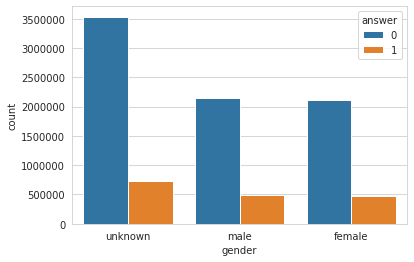
\includegraphics[width=\linewidth]{1.png}
  \caption{Gender}
  \Description{Gender}
\end{figure}

This feature has a total of 5 categories, [weekly, monthly, daily, new, unknown]. As can be seen from the histogram below, different categories have completely different distributions. This feature is obviously a very distinguishable feature.

\begin{figure}[H]
  \centering
  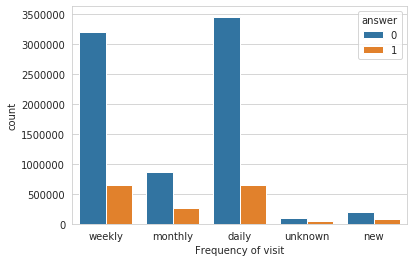
\includegraphics[width=\linewidth]{2.png}
  \caption{Frequency}
  \Description{Frequency}
\end{figure}

This feature is a two-category feature, and the following figure shows that the feature has a good degree of discrimination (the remaining two-category and multi-category features are the same, and will not be repeated).

\begin{figure}[H]
  \centering
  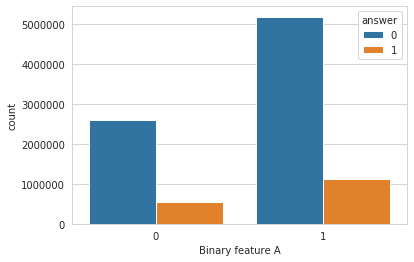
\includegraphics[width=\linewidth]{3.png}
  \caption{Binary feature A}
  \Description{Binary feature A}
\end{figure}


The code of data visualization is as follows:
\begin{lstlisting}
import matplotlib.pyplot as plt
import seaborn as sns

sns.set_style('whitegrid')

sns.countplot(x='gender',hue='answer',data=train)

#Out:<matplotlib.axes._subplots.AxesSubplot at 0x2ab9b576f290>

sns.countplot(x='Frequency of visit',hue='answer',data=train)

#Out:<matplotlib.axes._subplots.AxesSubplot at 0x2ab9a9974950>

sns.countplot(x='Binary feature A',hue='answer',data=train)

#Out:<matplotlib.axes._subplots.AxesSubplot at 0x2ab9ac8e5250>
\end{lstlisting}



\subsection{Feature Extraction}

In this part we merge the member information and the question information and invite information firstly.The code is as follows:
\begin{lstlisting}
train = pd.read_csv('invite_info_0926.txt', header=None, sep='\t')
train.columns = ['qid', 'uid', 'time','answer']
train = pd.merge(train, user_info, how='left', on='uid')
train = pd.merge(train, question_info, how='left', on='qid')
print(train.columns)

\end{lstlisting}

In this way, we get an initial train dataset, the index of it includes:


\begin{lstlisting}
Index(['qid', 'uid', 'time_x', 'answer', 'gender', 'keywords', 'number level',
       'Hotness level', 'Registration Type', 'Registration platform',
       'Frequency of visit', 'Binary feature A', 'Binary feature B',
       'Binary feature C', 'Binary feature D', 'Binary feature E',
       'Classification feature A ', 'Classification feature B',
       'Classification feature C', 'Classification feature D',
       'Classification feature E', 'Salt value', 'Follow topics',
       'Topic interested', 'time_y', 'title sig', 'title split ', 'des sig',
       'des split ', 'topic ids'],
      dtype='object')
\end{lstlisting}


Then, to utilize the feature of the member information of topics, we calulate the number, median number, max number and min number of member interested topics and some of other attributes. The code is as follows:
\begin{lstlisting}
member_info['num_atten_topic'] = member_info['topic_attent'].apply(len)
member_info['num_interest_topic'] = member_info['topic_interest'].apply(len)


def most_interest_topic(d):
    if len(d) == 0:
        return -1
    return list(d.keys())[np.argmax(list(d.values()))]




member_info['most_interest_topic'] = member_info['topic_interest'].apply(most_interest_topic)
member_info['most_interest_topic'] = LabelEncoder().fit_transform(member_info['most_interest_topic'])

def get_interest_values(d):
    if len(d) == 0:
        return [0]
    return list(d.values())


member_info['interest_values'] = member_info['topic_interest'].apply(get_interest_values)
member_info['min_interest_values'] = member_info['interest_values'].apply(np.min)
member_info['max_interest_values'] = member_info['interest_values'].apply(np.max)
member_info['mean_interest_values'] = member_info['interest_values'].apply(np.mean)
member_info['std_interest_values'] = member_info['interest_values'].apply(np.std)



def process(df):
    return df.apply(lambda row: [row['topic_interest'][t] for t in row['topic_interest_intersection']],axis=1)

pool = mp.Pool()
chunk_list = split_df(invite_id_qm, 100)
ret = pool.map(process, chunk_list)
invite_id_qm['topic_interest_intersection_values'] = pd.concat(ret)
gc_mp(pool, ret, chunk_list)





invite_id_qm['num_topic_attent_intersection'] = invite_id_qm['topic_attent_intersection'].apply(len)
invite_id_qm['num_topic_interest_intersection'] = invite_id_qm['topic_interest_intersection'].apply(len)



invite_id_qm['topic_interest_intersection_values'] = invite_id_qm['topic_interest_intersection_values'].apply(lambda x: [0] if len(x) == 0 else x)
invite_id_qm['min_topic_interest_intersection_values'] = invite_id_qm['topic_interest_intersection_values'].apply(np.min)
invite_id_qm['max_topic_interest_intersection_values'] = invite_id_qm['topic_interest_intersection_values'].apply(np.max)
invite_id_qm['mean_topic_interest_intersection_values'] = invite_id_qm['topic_interest_intersection_values'].apply(np.mean)
invite_id_qm['std_topic_interest_intersection_values'] = invite_id_qm['topic_interest_intersection_values'].apply(np.std)

feats = ['author_question_id', 'num_topic_attent_intersection', 'num_topic_interest_intersection', 'min_topic_interest_intersection_values', 'max_topic_interest_intersection_values', 'mean_topic_interest_intersection_values', 'std_topic_interest_intersection_values']
feats += []
member_question_feat = invite_id_qm[feats]
\end{lstlisting}

At last, we encode other features.Related function code is as follows:
\begin{lstlisting}
def parse_str(d):
    return np.array(list(map(float, d.split())))

def parse_list_1(d):
    if d == '-1':
        return [0]
    return list(map(lambda x: int(x[1:]), str(d).split(',')))

def parse_list_2(d):
    if d == '-1':
        return [0]
    return list(map(lambda x: int(x[2:]), str(d).split(',')))

def parse_map(d):
    if d == '-1':
        return {}
    return dict([int(z.split(':')[0][1:]), float(z.split(':')[1])] for z in d.split(','))
\end{lstlisting}



%%%%%%%%%%%%%%%%%%%%%%%%%%%%%%%%%%%%%%%%%%%%%%%%%%%%%%%%%%%%%%%%%%%%%%%%%%%%%%%%%%%%

\section{Classifier}

In this competition, I used the XGboost Classifier and LGBM Classifier. In this section, I will introduce these two Classifiers and introduce how I used them.

\subsection{XGboost}


XGBoostis an open-source software library which provides a gradient boosting framework for C++, Java, Python. It works on Linux, Windows,and macOS. From the project description, it aims to provide a "Scalable, Portable and Distributed Gradient Boosting (GBM, GBRT, GBDT) Library". It runs on a single machine, as well as the distributed processing frameworks Apache Hadoop, Apache Spark, and Apache Flink. It has gained much popularity and attention recently as the algorithm of choice for many winning teams of machine learning competitions.

Compared to other traditional classifier, we have to transform the data from array form to Dmatrix form. The code of it is as follows:
\begin{lstlisting}
import xgboost as xgb
from sklearn.metrics import accuracy_score
import scipy

dtrain = xgb.DMatrix( X_train, label=y_train)
dval=xgb.DMatrix( X_val, label=y_val)
\end{lstlisting}

There are many parameters should be adjusted, here are some important paramaters:

\begin{itemize}
\item \textit{objective}

Specify the learning task and the corresponding learning objective. The objective options are below:
	\subitem reg:squarederror
	\subitem reg:squaredlogerror
	\subitem reg:logistic
	\subitem $\cdots$
	\subitem binary:logistic
	\subitem multi:softmax
In this competition, I will definitely choose the"binary:logistic",because I need to give the probability of binary classfication qusetion.

\item \textit{gamma}

Gamma is the minimum loss reduction required to make a further partition on a leaf node of the tree. The larger gamma is, the more conservative the algorithm will be. In my program,I choose $0.1$as my gamma

\item \textit{max depth}

Maximum depth of a tree. Increasing this value will make the model more complex and more likely to overfit. 0 is only accepted in lossguided growing policy when tree-method is set as hist and it indicates no limit on depth. Beware that XGBoost aggressively consumes memory when training a deep tree.During the process of my preparing for the competition,I found this is the most influential paramater in all paramaters. Finally, I choose 8 as my max depth.

\item \textit{lambda}

L2 regularization term on weights. Increasing this value will make model more conservative.I choose 2 as my max lambda.

\item \textit{tree method}

XGBoost supports approx, hist and gpu hist for distributed training. Experimental support for external memory is available for approx and gpu hist.Because my server has a NVIDIA GPU, I choose the "gpu hist",whose training is much faster than CPU.

\end{itemize}


Code of this part is as follows:

\begin{lstlisting}
num_round = 5000
params = {
    'booster': 'gbtree',
    'objective': 'binary:logistic',  
    'gamma': 0.1,                 
    'max_depth': 8,               
    'lambda': 2,                   
    'subsample': 0.8,              
    'colsample_bytree': 0.8,       
    'min_child_weight': 3,
    'silent': 0,                   
    'eta': 0.002,                  
    'seed': 1000,
    'tree_method':'gpu_hist',
    'predictor':'gpu_predictor',
    'eval_metric': ['logloss', 'error', 'auc'],
    'verbose_eval':True,
    
    
}



bst = xgb.train( params, dtrain, num_round, evals=[(dval,'evl')])
dtest = xgb.DMatrix(test[feature_cols])
ans1 = bst.predict(dtest)


\end{lstlisting}

\subsection{LGBM}

LightGBM is a gradient boosting framework that uses tree based learning algorithms. It is designed to be distributed and efficient with the following advantages:

\begin{itemize}
\item Faster training speed and higher efficiency.
\item Lower memory usage.
\item Better accuracy.
\item Support of parallel and GPU learning.
\item Capable of handling large-scale data.

\end{itemize}

Code of this part is as follows:
\begin{lstlisting}
model_lgb = LGBMClassifier(n_estimators=2000, n_jobs=-1, objective='binary', seed=1000, silent=True)
model_lgb.fit(X_train, y_train,
              eval_metric=['logloss', 'auc'],
              eval_set=[(X_val, y_val)],
              early_stopping_rounds=50)
ans2= model_lgb.predict_proba(test[feature_cols])[:, 1]
\end{lstlisting}

\section{Result and Summary}

In the end, my online accuracy rate reached \textbf{81.542\%}, ranking \textbf{62th} among all the contestants, and ranking \textbf{1st} among the students who chose this competition in the "Information Retrieval and Data Mining" class.


By taking part in this competition, I can skillfully use LGBM and XGboost classifiers. And it improved my inderstanding of machine learing and data mining. Although finally I haven't won any awards, I think I still benefit a lot from \textit{BAAI-ZHIHU Expert Finding Competition}


\section{Acknowledgments}

I would like to extend my sincere gratitude to my supervisor, \textbf{Prof. Jianhua Yin}, for your instructive advice and useful suggestions on my thesis. I am deeply grateful of your help in the completion of this thesis.



\end{document}
\endinput
%%
%% End of file `sample-sigconf.tex'.
